\documentclass{book}
\usepackage[a4paper,margin=1cm]{geometry}
\usepackage{tikz}
\usepackage{verbatim}
\begin{document}
\section{priorité fixe}
\begin{table}[!h]
\begin{center}
\begin{tabular}{|c|c|c|c|}
 \hline$\tau_i$ & $C_i$ & $D_i$ & $T_i$ \\ 
 \hline1 & 5 & 10 & 10 \\ 
 \hline 2 & 7 & 15 & 21 \\ 
 \hline 3 & 2 & 22 & 24 \\ 
 \hline 
 \end{tabular}
\end{center}
\caption{Ensemble de tâche périodique} \label{tab:dmmp}
\end{table}
\section{insertion locale}
\begin{figure}[!h]
\begin{center}
\resizebox{15cm}{4cm}{
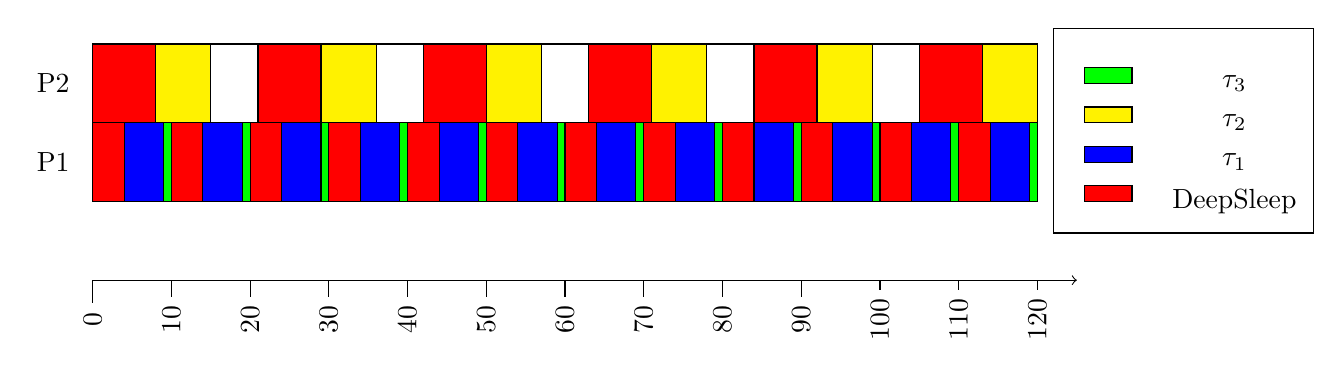
\begin{tikzpicture}
\node at (-0.5,0.5) {P1};
\node at (-0.5,1.5) {P2};
%P1 DS
\draw[fill=red] (0,0) rectangle (0.4,1) ;
\draw[fill=red] (1,0) rectangle (1.4,1) ;
\draw[fill=red] (2,0) rectangle (2.4,1) ;
\draw[fill=red] (3,0) rectangle (3.4,1) ;
\draw[fill=red] (4,0) rectangle (4.4,1) ;
\draw[fill=red] (5,0) rectangle (5.4,1) ;
\draw[fill=red] (6,0) rectangle (6.4,1) ;
\draw[fill=red] (7,0) rectangle (7.4,1) ;
\draw[fill=red] (8,0) rectangle (8.4,1) ;
\draw[fill=red] (9,0) rectangle (9.4,1) ;
\draw[fill=red] (10,0) rectangle (10.4,1) ;
\draw[fill=red] (11,0) rectangle (11.4,1) ;
%P1 T1
\draw[fill=blue] (0.4,0) rectangle (0.9,1) ;
\draw[fill=blue] (1.4,0) rectangle (1.9,1) ;
\draw[fill=blue] (2.4,0) rectangle (2.9,1) ;
\draw[fill=blue] (3.4,0) rectangle (3.9,1) ;
\draw[fill=blue] (4.4,0) rectangle (4.9,1) ;
\draw[fill=blue] (5.4,0) rectangle (5.9,1) ;
\draw[fill=blue] (6.4,0) rectangle (6.9,1) ;
\draw[fill=blue] (7.4,0) rectangle (7.9,1) ;
\draw[fill=blue] (8.4,0) rectangle (8.9,1) ;
\draw[fill=blue] (9.4,0) rectangle (9.9,1) ;
\draw[fill=blue] (10.4,0) rectangle (10.9,1) ;
\draw[fill=blue] (11.4,0) rectangle (11.9,1) ;
%P1 T3
\draw[fill=green] (0.9,0) rectangle (1,1) ;
\draw[fill=green] (1.9,0) rectangle (2,1) ;
\draw[fill=green] (2.9,0) rectangle (3,1) ;
\draw[fill=green] (3.9,0) rectangle (4,1) ;
\draw[fill=green] (4.9,0) rectangle (5,1) ;
\draw[fill=green] (5.9,0) rectangle (6,1) ;
\draw[fill=green] (6.9,0) rectangle (7,1) ;
\draw[fill=green] (7.9,0) rectangle (8,1) ;
\draw[fill=green] (8.9,0) rectangle (9,1) ;
\draw[fill=green] (9.9,0) rectangle (10,1) ;
\draw[fill=green] (10.9,0) rectangle (11,1) ;
\draw[fill=green] (11.9,0) rectangle (12,1) ;

\draw[fill=red] (0.0,1) rectangle (0.8,2) ;
\draw[fill=yellow] (0.8,1) rectangle (1.5,2) ;
\draw[fill=white] (1.5,1) rectangle (2.1,2) ;

\draw[fill=red] (2.1,1) rectangle (2.899999904632568,2) ;
\draw[fill=yellow] (2.899999904632568,1) rectangle (3.5999999046325684,2) ;
\draw[fill=white] (3.5999999046325684,1) rectangle (4.199999904632568,2) ;

\draw[fill=red] (4.2,1) rectangle (4.9999998092651365,2) ;
\draw[fill=yellow] (4.9999998092651365,1) rectangle (5.699999809265137,2) ;
\draw[fill=white] (5.699999809265137,1) rectangle (6.299999809265136,2) ;

\draw[fill=red] (6.2999997,1) rectangle (7.099999713897705,2) ;
\draw[fill=yellow] (7.099999713897705,1) rectangle (7.799999713897705,2) ;
\draw[fill=white] (7.799999713897705,1) rectangle (8.399999713897705,2) ;

\draw[fill=red] (8.4,1) rectangle (9.199999618530274,2) ;
\draw[fill=yellow] (9.199999618530274,1) rectangle (9.899999618530273,2) ;
\draw[fill=white] (9.899999618530273,1) rectangle (10.499999618530273,2) ;

\draw[fill=red] (10.5,1) rectangle (11.3,2) ;
\draw[fill=yellow] (11.3,1) rectangle (12.0,2) ;

\draw [->](0,-1) -- coordinate (x axis mid) (12.5,-1);
\draw (0,-1) -- (0,-1.5) node[fill=white,rotate=90] {0};
\draw (1,-1) -- (1,-1.5) node[fill=white,rotate=90] {10};
\draw (2,-1) -- (2,-1.5) node[fill=white,rotate=90] {20};
\draw (3,-1) -- (3,-1.5) node[fill=white,rotate=90] {30};
\draw (4,-1) -- (4,-1.5) node[fill=white,rotate=90] {40};
\draw (5,-1) -- (5,-1.5) node[fill=white,rotate=90] {50};
\draw (6,-1) -- (6,-1.5) node[fill=white,rotate=90] {60};
\draw (7,-1) -- (7,-1.5) node[fill=white,rotate=90] {70};
\draw (8,-1) -- (8,-1.5) node[fill=white,rotate=90] {80};
\draw (9,-1) -- (9,-1.5) node[fill=white,rotate=90] {90};
\draw (10,-1) -- (10,-1.5) node[fill=white,rotate=90] {100};
\draw (11,-1) -- (11,-1.5) node[fill=white,rotate=90] {110};
\draw (12,-1) -- (12,-1.5) node[fill=white,rotate=90] {120};

\draw[fill=white] (12.2,-0.4) rectangle (15.5,2.2) ;
\draw[fill=red] (12.6,0) rectangle (13.2,0.2) ;
\draw (14.5,0) -- (14.5,0) node[fill=white] {DeepSleep};
\draw[fill=blue] (12.6,0.5) rectangle (13.2,0.7) ;
\draw (14.5,0.5) -- (14.5,0.5) node[fill=white] {$\tau_1$};
\draw[fill=yellow] (12.6,1) rectangle (13.2,1.2) ;
\draw (14.5,1) -- (14.5,1) node[fill=white] {$\tau_2$};
\draw[fill=green] (12.6,1.5) rectangle (13.2,1.7) ;
\draw (14.5,1.5) -- (14.5,1.5) node[fill=white] {$\tau_3$};
\end{tikzpicture}}
\end{center}
\caption{Insertion locale de tâches d'endormissements dans un multiprocesseur} \label{fig:dmmpl}
\end{figure}
\section{insertion globale}
\begin{figure}[!h]
\begin{center}
\resizebox{15cm}{4cm}{
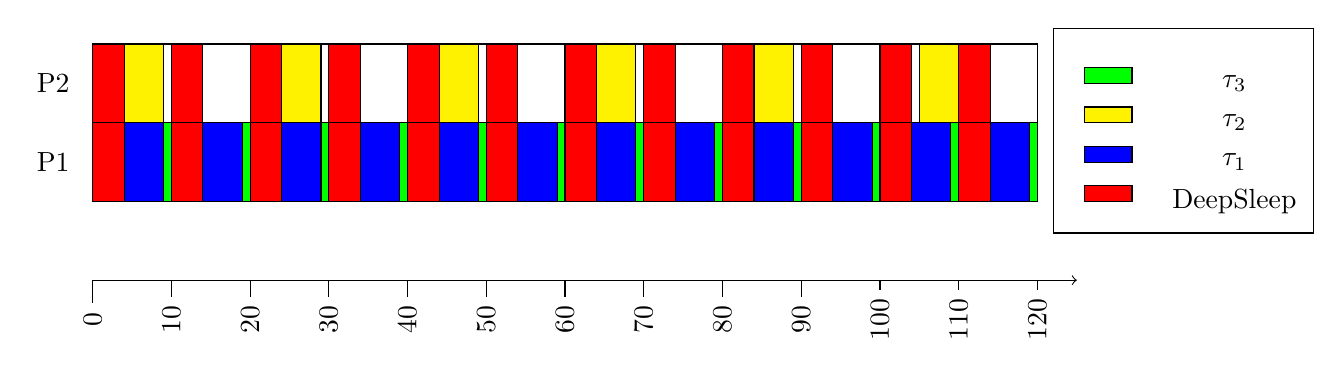
\begin{tikzpicture}
\node at (-0.5,0.5) {P1};
\node at (-0.5,1.5) {P2};
%P1 DS
\draw[fill=red] (0,0) rectangle (0.4,1) ;
\draw[fill=red] (1,0) rectangle (1.4,1) ;
\draw[fill=red] (2,0) rectangle (2.4,1) ;
\draw[fill=red] (3,0) rectangle (3.4,1) ;
\draw[fill=red] (4,0) rectangle (4.4,1) ;
\draw[fill=red] (5,0) rectangle (5.4,1) ;
\draw[fill=red] (6,0) rectangle (6.4,1) ;
\draw[fill=red] (7,0) rectangle (7.4,1) ;
\draw[fill=red] (8,0) rectangle (8.4,1) ;
\draw[fill=red] (9,0) rectangle (9.4,1) ;
\draw[fill=red] (10,0) rectangle (10.4,1) ;
\draw[fill=red] (11,0) rectangle (11.4,1) ;
%P1 T1
\draw[fill=blue] (0.4,0) rectangle (0.9,1) ;
\draw[fill=blue] (1.4,0) rectangle (1.9,1) ;
\draw[fill=blue] (2.4,0) rectangle (2.9,1) ;
\draw[fill=blue] (3.4,0) rectangle (3.9,1) ;
\draw[fill=blue] (4.4,0) rectangle (4.9,1) ;
\draw[fill=blue] (5.4,0) rectangle (5.9,1) ;
\draw[fill=blue] (6.4,0) rectangle (6.9,1) ;
\draw[fill=blue] (7.4,0) rectangle (7.9,1) ;
\draw[fill=blue] (8.4,0) rectangle (8.9,1) ;
\draw[fill=blue] (9.4,0) rectangle (9.9,1) ;
\draw[fill=blue] (10.4,0) rectangle (10.9,1) ;
\draw[fill=blue] (11.4,0) rectangle (11.9,1) ;
%P1 T3
\draw[fill=green] (0.9,0) rectangle (1,1) ;
\draw[fill=green] (1.9,0) rectangle (2,1) ;
\draw[fill=green] (2.9,0) rectangle (3,1) ;
\draw[fill=green] (3.9,0) rectangle (4,1) ;
\draw[fill=green] (4.9,0) rectangle (5,1) ;
\draw[fill=green] (5.9,0) rectangle (6,1) ;
\draw[fill=green] (6.9,0) rectangle (7,1) ;
\draw[fill=green] (7.9,0) rectangle (8,1) ;
\draw[fill=green] (8.9,0) rectangle (9,1) ;
\draw[fill=green] (9.9,0) rectangle (10,1) ;
\draw[fill=green] (10.9,0) rectangle (11,1) ;
\draw[fill=green] (11.9,0) rectangle (12,1) ;

\draw[fill=white] (0,1) rectangle (12,2) ;
\draw[fill=red] (0,1) rectangle (0.4,2) ;
\draw[fill=red] (1,1) rectangle (1.4,2) ;
\draw[fill=red] (2,1) rectangle (2.4,2) ;
\draw[fill=red] (3,1) rectangle (3.4,2) ;
\draw[fill=red] (4,1) rectangle (4.4,2) ;
\draw[fill=red] (5,1) rectangle (5.4,2) ;
\draw[fill=red] (6,1) rectangle (6.4,2) ;
\draw[fill=red] (7,1) rectangle (7.4,2) ;
\draw[fill=red] (8,1) rectangle (8.4,2) ;
\draw[fill=red] (9,1) rectangle (9.4,2) ;
\draw[fill=red] (10,1) rectangle (10.4,2) ;
\draw[fill=red] (11,1) rectangle (11.4,2) ;

\draw[fill=yellow] (0.4,1) rectangle (0.9,2) ;
\draw[fill=yellow] (2.4,1) rectangle (2.9,2) ;
\draw[fill=yellow] (4.4,1) rectangle (4.9,2) ;
\draw[fill=yellow] (6.4,1) rectangle (6.9,2) ;
\draw[fill=yellow] (8.4,1) rectangle (8.9,2) ;
\draw[fill=yellow] (10.5,1) rectangle (11,2) ;



\draw [->](0,-1) -- coordinate (x axis mid) (12.5,-1);
\draw (0,-1) -- (0,-1.5) node[fill=white,rotate=90] {0};
\draw (1,-1) -- (1,-1.5) node[fill=white,rotate=90] {10};
\draw (2,-1) -- (2,-1.5) node[fill=white,rotate=90] {20};
\draw (3,-1) -- (3,-1.5) node[fill=white,rotate=90] {30};
\draw (4,-1) -- (4,-1.5) node[fill=white,rotate=90] {40};
\draw (5,-1) -- (5,-1.5) node[fill=white,rotate=90] {50};
\draw (6,-1) -- (6,-1.5) node[fill=white,rotate=90] {60};
\draw (7,-1) -- (7,-1.5) node[fill=white,rotate=90] {70};
\draw (8,-1) -- (8,-1.5) node[fill=white,rotate=90] {80};
\draw (9,-1) -- (9,-1.5) node[fill=white,rotate=90] {90};
\draw (10,-1) -- (10,-1.5) node[fill=white,rotate=90] {100};
\draw (11,-1) -- (11,-1.5) node[fill=white,rotate=90] {110};
\draw (12,-1) -- (12,-1.5) node[fill=white,rotate=90] {120};

\draw[fill=white] (12.2,-0.4) rectangle (15.5,2.2) ;
\draw[fill=red] (12.6,0) rectangle (13.2,0.2) ;
\draw (14.5,0) -- (14.5,0) node[fill=white] {DeepSleep};
\draw[fill=blue] (12.6,0.5) rectangle (13.2,0.7) ;
\draw (14.5,0.5) -- (14.5,0.5) node[fill=white] {$\tau_1$};
\draw[fill=yellow] (12.6,1) rectangle (13.2,1.2) ;
\draw (14.5,1) -- (14.5,1) node[fill=white] {$\tau_2$};
\draw[fill=green] (12.6,1.5) rectangle (13.2,1.7) ;
\draw (14.5,1.5) -- (14.5,1.5) node[fill=white] {$\tau_3$};
\end{tikzpicture}}
\end{center}
\caption{Insertion globale de tâches d'endormissements dans un multiprocesseur} \label{fig:dmmpg}
\end{figure}
\section{dynamique}
\begin{table}[h]
\begin{center}
\begin{tabular}{|c|c|c|c|}
 \hline$\tau_i$ & $C_i$ & $D_i$ & $T_i$ \\ 
 \hline1 & 2 & 10 & 10 \\ 
 \hline 2 & 2 & 15 & 21 \\ 
 \hline 
 \end{tabular}
\end{center}
\caption{Insertion locale de tâches d'endormissements dans un multiprocesseur} \label{tab:edfmp}
\end{table}
\section{insertion locale}
\begin{figure}[!h]
\begin{center}
\resizebox{15cm}{4cm}{
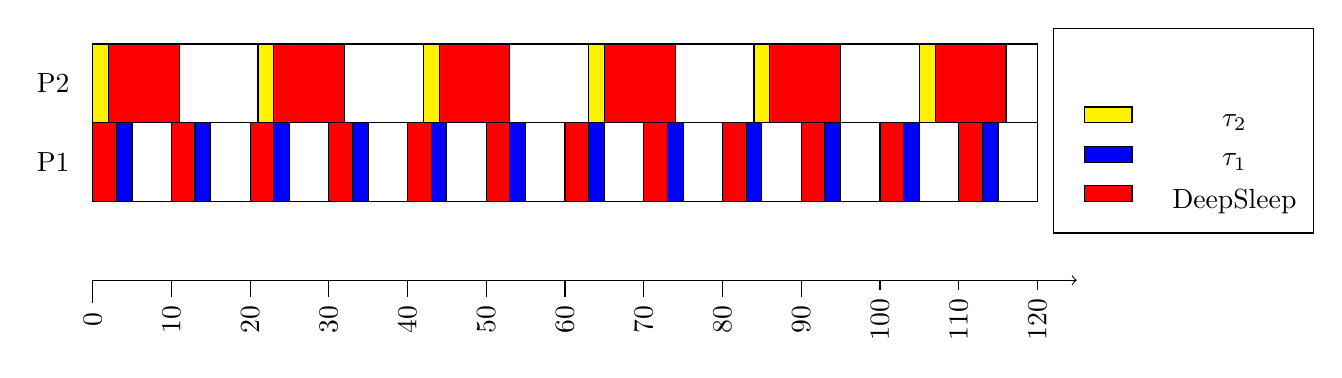
\begin{tikzpicture}
\node at (-0.5,0.5) {P1};
\node at (-0.5,1.5) {P2};
%P1
\draw[fill=white] (0.0,0) rectangle (12,1) ;

\draw[fill=red] (0.0,0) rectangle (0.3,1) ;
\draw[fill=blue] (0.3,0) rectangle (0.5,1) ;

\draw[fill=red] (1.0,0) rectangle (1.3,1) ;
\draw[fill=blue] (1.3,0) rectangle (1.5,1) ;

\draw[fill=red] (2.0,0) rectangle (2.3,1) ;
\draw[fill=blue] (2.3,0) rectangle (2.5,1) ;

\draw[fill=red] (3.0,0) rectangle (3.3,1) ;
\draw[fill=blue] (3.3,0) rectangle (3.5,1) ;

\draw[fill=red] (4.0,0) rectangle (4.3,1) ;
\draw[fill=blue] (4.3,0) rectangle (4.5,1) ;

\draw[fill=red] (5.0,0) rectangle (5.3,1) ;
\draw[fill=blue] (5.3,0) rectangle (5.5,1) ;

\draw[fill=red] (6.0,0) rectangle (6.3,1) ;
\draw[fill=blue] (6.3,0) rectangle (6.5,1) ;

\draw[fill=red] (7.0,0) rectangle (7.3,1) ;
\draw[fill=blue] (7.3,0) rectangle (7.5,1) ;

\draw[fill=red] (8.0,0) rectangle (8.3,1) ;
\draw[fill=blue] (8.3,0) rectangle (8.5,1) ;

\draw[fill=red] (9.0,0) rectangle (9.3,1) ;
\draw[fill=blue] (9.3,0) rectangle (9.5,1) ;

\draw[fill=red] (10.0,0) rectangle (10.3,1) ;
\draw[fill=blue] (10.3,0) rectangle (10.5,1) ;

\draw[fill=red] (11.0,0) rectangle (11.3,1) ;
\draw[fill=blue] (11.3,0) rectangle (11.5,1) ;
%P2
\draw[fill=white] (0.0,1) rectangle (12,2) ;

\draw[fill=yellow] (0.0,1) rectangle (0.2,2) ;
\draw[fill=red] (0.2,1) rectangle (1.1,2) ;

\draw[fill=yellow] (2.1,1) rectangle (2.2999999046325685,2) ;
\draw[fill=red] (2.2999999046325685,1) rectangle (3.1999999046325684,2) ;

\draw[fill=yellow] (4.2,1) rectangle (4.399999809265137,2) ;
\draw[fill=red] (4.399999809265137,1) rectangle (5.299999809265136,2) ;

\draw[fill=yellow] (6.2999997,1) rectangle (6.499999713897705,2) ;
\draw[fill=red] (6.499999713897705,1) rectangle (7.399999713897705,2) ;

\draw[fill=yellow] (8.4,1) rectangle (8.599999618530273,2) ;
\draw[fill=red] (8.599999618530273,1) rectangle (9.499999618530273,2) ;

\draw[fill=yellow] (10.5,1) rectangle (10.7,2) ;
\draw[fill=red] (10.7,1) rectangle (11.6,2) ;
%%%%%%%
\draw [->](0,-1) -- coordinate (x axis mid) (12.5,-1);
\draw (0,-1) -- (0,-1.5) node[fill=white,rotate=90] {0};
\draw (1,-1) -- (1,-1.5) node[fill=white,rotate=90] {10};
\draw (2,-1) -- (2,-1.5) node[fill=white,rotate=90] {20};
\draw (3,-1) -- (3,-1.5) node[fill=white,rotate=90] {30};
\draw (4,-1) -- (4,-1.5) node[fill=white,rotate=90] {40};
\draw (5,-1) -- (5,-1.5) node[fill=white,rotate=90] {50};
\draw (6,-1) -- (6,-1.5) node[fill=white,rotate=90] {60};
\draw (7,-1) -- (7,-1.5) node[fill=white,rotate=90] {70};
\draw (8,-1) -- (8,-1.5) node[fill=white,rotate=90] {80};
\draw (9,-1) -- (9,-1.5) node[fill=white,rotate=90] {90};
\draw (10,-1) -- (10,-1.5) node[fill=white,rotate=90] {100};
\draw (11,-1) -- (11,-1.5) node[fill=white,rotate=90] {110};
\draw (12,-1) -- (12,-1.5) node[fill=white,rotate=90] {120};

\draw[fill=white] (12.2,-0.4) rectangle (15.5,2.2) ;
\draw[fill=red] (12.6,0) rectangle (13.2,0.2) ;
\draw (14.5,0) -- (14.5,0) node[fill=white] {DeepSleep};
\draw[fill=blue] (12.6,0.5) rectangle (13.2,0.7) ;
\draw (14.5,0.5) -- (14.5,0.5) node[fill=white] {$\tau_1$};
\draw[fill=yellow] (12.6,1) rectangle (13.2,1.2) ;
\draw (14.5,1) -- (14.5,1) node[fill=white] {$\tau_2$};
\end{tikzpicture}}
\end{center}
\caption{Insertion globale de tâches d'endormissements dans un multiprocesseur} \label{fig:edfmpl}
\end{figure}
\section{insertion globale}
\begin{figure}[!h]
\begin{center}
\resizebox{15cm}{4cm}{
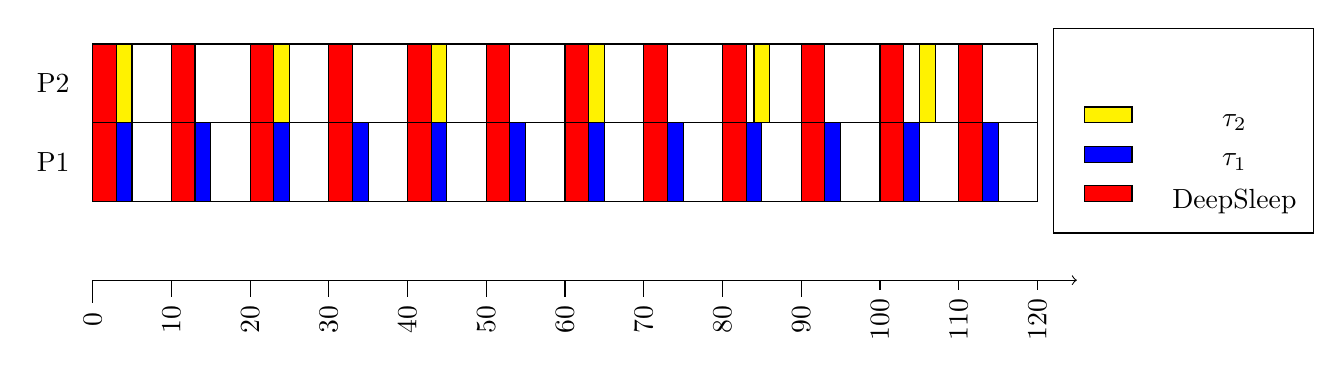
\begin{tikzpicture}
\node at (-0.5,0.5) {P1};
\node at (-0.5,1.5) {P2};
%P1
\draw[fill=white] (0.0,0) rectangle (12,1) ;

\draw[fill=red] (0.0,0) rectangle (0.3,1) ;
\draw[fill=blue] (0.3,0) rectangle (0.5,1) ;

\draw[fill=red] (1.0,0) rectangle (1.3,1) ;
\draw[fill=blue] (1.3,0) rectangle (1.5,1) ;

\draw[fill=red] (2.0,0) rectangle (2.3,1) ;
\draw[fill=blue] (2.3,0) rectangle (2.5,1) ;

\draw[fill=red] (3.0,0) rectangle (3.3,1) ;
\draw[fill=blue] (3.3,0) rectangle (3.5,1) ;

\draw[fill=red] (4.0,0) rectangle (4.3,1) ;
\draw[fill=blue] (4.3,0) rectangle (4.5,1) ;

\draw[fill=red] (5.0,0) rectangle (5.3,1) ;
\draw[fill=blue] (5.3,0) rectangle (5.5,1) ;

\draw[fill=red] (6.0,0) rectangle (6.3,1) ;
\draw[fill=blue] (6.3,0) rectangle (6.5,1) ;

\draw[fill=red] (7.0,0) rectangle (7.3,1) ;
\draw[fill=blue] (7.3,0) rectangle (7.5,1) ;

\draw[fill=red] (8.0,0) rectangle (8.3,1) ;
\draw[fill=blue] (8.3,0) rectangle (8.5,1) ;

\draw[fill=red] (9.0,0) rectangle (9.3,1) ;
\draw[fill=blue] (9.3,0) rectangle (9.5,1) ;

\draw[fill=red] (10.0,0) rectangle (10.3,1) ;
\draw[fill=blue] (10.3,0) rectangle (10.5,1) ;

\draw[fill=red] (11.0,0) rectangle (11.3,1) ;
\draw[fill=blue] (11.3,0) rectangle (11.5,1) ;
%P2
\draw[fill=white] (0.0,1) rectangle (12,2) ;

\draw[fill=red] (0.0,1) rectangle (0.3,2) ;
\draw[fill=red] (1.0,1) rectangle (1.3,2) ;
\draw[fill=red] (2.0,1) rectangle (2.3,2) ;
\draw[fill=red] (3.0,1) rectangle (3.3,2) ;
\draw[fill=red] (4.0,1) rectangle (4.3,2) ;
\draw[fill=red] (5.0,1) rectangle (5.3,2) ;
\draw[fill=red] (6.0,1) rectangle (6.3,2) ;
\draw[fill=red] (7.0,1) rectangle (7.3,2) ;
\draw[fill=red] (8.0,1) rectangle (8.3,2) ;
\draw[fill=red] (9.0,1) rectangle (9.3,2) ;
\draw[fill=red] (10.0,1) rectangle (10.3,2) ;
\draw[fill=red] (11.0,1) rectangle (11.3,2) ;

\draw[fill=yellow] (0.3,1) rectangle (0.5,2) ;
\draw[fill=yellow] (2.3,1) rectangle (2.5,2) ;
\draw[fill=yellow] (4.3,1) rectangle (4.5,2) ;
\draw[fill=yellow] (6.3,1) rectangle (6.5,2) ;
\draw[fill=yellow] (8.4,1) rectangle (8.6,2) ;
\draw[fill=yellow] (10.5,1) rectangle (10.7,2) ;
%%%%%%%
\draw [->](0,-1) -- coordinate (x axis mid) (12.5,-1);
\draw (0,-1) -- (0,-1.5) node[fill=white,rotate=90] {0};
\draw (1,-1) -- (1,-1.5) node[fill=white,rotate=90] {10};
\draw (2,-1) -- (2,-1.5) node[fill=white,rotate=90] {20};
\draw (3,-1) -- (3,-1.5) node[fill=white,rotate=90] {30};
\draw (4,-1) -- (4,-1.5) node[fill=white,rotate=90] {40};
\draw (5,-1) -- (5,-1.5) node[fill=white,rotate=90] {50};
\draw (6,-1) -- (6,-1.5) node[fill=white,rotate=90] {60};
\draw (7,-1) -- (7,-1.5) node[fill=white,rotate=90] {70};
\draw (8,-1) -- (8,-1.5) node[fill=white,rotate=90] {80};
\draw (9,-1) -- (9,-1.5) node[fill=white,rotate=90] {90};
\draw (10,-1) -- (10,-1.5) node[fill=white,rotate=90] {100};
\draw (11,-1) -- (11,-1.5) node[fill=white,rotate=90] {110};
\draw (12,-1) -- (12,-1.5) node[fill=white,rotate=90] {120};

\draw[fill=white] (12.2,-0.4) rectangle (15.5,2.2) ;
\draw[fill=red] (12.6,0) rectangle (13.2,0.2) ;
\draw (14.5,0) -- (14.5,0) node[fill=white] {DeepSleep};
\draw[fill=blue] (12.6,0.5) rectangle (13.2,0.7) ;
\draw (14.5,0.5) -- (14.5,0.5) node[fill=white] {$\tau_1$};
\draw[fill=yellow] (12.6,1) rectangle (13.2,1.2) ;
\draw (14.5,1) -- (14.5,1) node[fill=white] {$\tau_2$};
\end{tikzpicture}}
\end{center}
\caption{} \label{fig:edfmpg}
\end{figure}
\end{document}